%srj
%aum gaanathipathaye namaha
\section{Selective Inlining}\label{sec:inline}
In this section, we explain the approach of selective inlining, which helps to extract the true semantics of the functions under investigation, via the function coupling analysis.
%The blindly inlining strategy would lead to such a problem of code size explosion that the bloated functions are hard to analyze, incurring heavy overhead.
%However, one might assume that inlining all the callee functions at their respective call sites, as in~\cite{wang2015binary}, would solve the partial (or incomplete) semantics problem present in existing binary function matching techniques.
To overcome C3, a systematic approach is desirable to decide which target functions to be inlined --- a fundamental problem also faced by the compilers, where they have to decide what functions need to be inlined, during the compilation process, in order to optimize the binaries for maximum speed or minimum size~\cite{chang1992profile}. 
However, binary code search and compilation have different goals for inlining decision. Compilers have access to high-level programming constructs from source code and their inlining decision is influenced by various factors such as user-defined \mahin{\texttt{INLINE} pragmas}, target function body-size, call-size (i.e., overhead required to invoke the function), saving estimation (i.e., estimated shrink in binary after inline), effects on caching, paging and register pressure~\cite{chang1992profile}. On the contrary, in binary code search, 
inlining decision needs to made with the minimum information available from the stripped binaries and make inlining decision. With the hope to capture the true semantics of the functions, selective inlining for binary analysis has yet to attain the scalability.}

\subsection{Caller-callee Relationship Patterns}

\begin{figure*}[ht]
   \centering
   %height=5cm,width=0.8\textwidth
  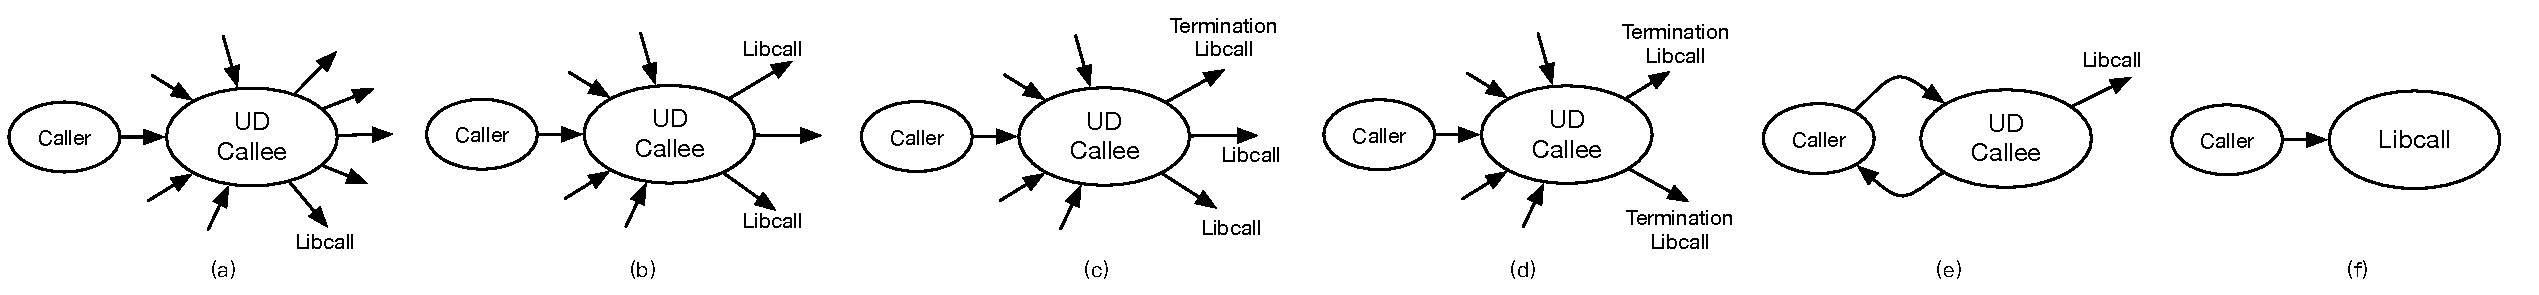
\includegraphics[width=\textwidth]{srj-figures/srj-caller-callee3.pdf}
  %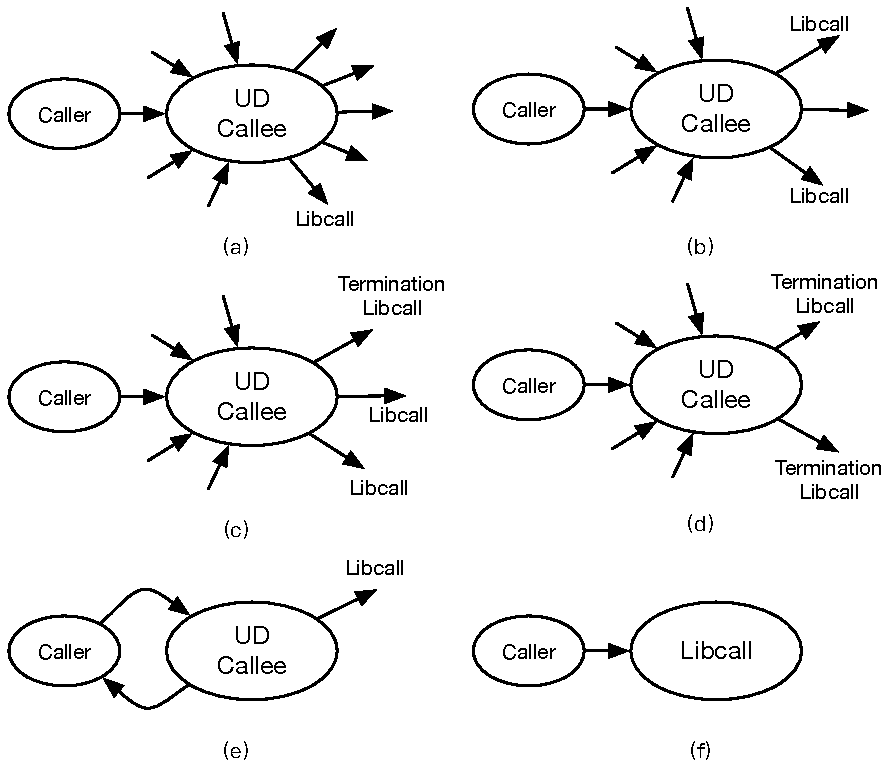
\includegraphics[width=0.45\textwidth]{srj-figures/srj-caller-callee4.pdf}
  \caption{Commonly observed callar-callee relationship patterns, where `UD callee' denotes user-defined called fucntion.} \label{fig:caller-callee}
\end{figure*}

%In contrast to compilers,
\xyx{In order to inline those commonly used ones, we use the caller-callee relationship to guide the inlining decision. According to our empirical study on XX, seven commonly-observed caller-callee relationship patterns are identified and summarised in Fig.~\ref{fig:caller-callee}.}

Incoming and outgoing edges in Fig \ref{fig:caller-callee} represent  the incoming and outgoing calls to function(s) from the function, respectively. \xyx{?? out of six patterns refer to the functions to be inlined, while ?? others are not. Here, we explain some typical patterns in details.}

\xyx{\noindent\textbf{Inlining case 1:} Fig~\ref{fig:caller-callee}(f) depicts the direct invocation of library function by the function $f_1$ under investigation. The case of $f_1$ indicates a \textit{wrap function} of certain library function, which helps to recover the semantics of $f_1$ via the semantics of called library function.  Currernt, we consider only the most common library functions --- 60 library functions, from both Linux (\texttt{libc}) and Windows (\texttt{msvcrt}), e.g., \texttt{memcpy} and \texttt{strlen} for inlining. However, we don't see any limitation in adding more library functions to this list.}

\xyx{\noindent\textbf{Inlining case 2:} Fig~\ref{fig:caller-callee}(e) depicts the case of a recursive relationship between the caller and callee $f_2$, where $f_2$ calls a library function. We consider this case is an recursive version of inlining case 1, so we also inline $f_2$ into its caller. Note that the recursive functions are, unlike that in compilers~\cite{chang1992profile} \textbf{??Mahin, how many times for compilers}, inlined only once for recursion.}

\xyx{\noindent\textbf{Inlining case 3:} Fig~\ref{fig:caller-callee}(b) depicts a common inlining case of the \textit{utility function} --- e.g., the UD (user-defined) function $f_3$ is called by many other UD functions, while $f_3$ calls several \textit{library or system functions} and few (or zero) UD functions. It suggests that $f_3$ is behaving as a utility function and hence, and $f_3$ has some semantics that is commonly needed by other functions.} % depending on the number of other UD functions `referred to' by this callee (lower the reference to other UD functions, better chance of inlining).}

\xyx{\noindent\textbf{Inlining case 4:} $f_4$ in Fig~\ref{fig:caller-callee}(c) is a variant of (b), where it has only reference to library functions and \textit{zero} reference to other UD functions. Such zero reference to UD functions indicates $f_4$ carries some unique semantics --- called \textit{unique function}, an ideal candidate for inlining. Note that $f_4$ is inlined as the majority of its invoked library functions are not of termination type. \textbf{Mahin, explain why termination type matters}}


\xyx{\noindent\textbf{Non-inlining case 1:} In Fig~\ref{fig:caller-callee}(d), $f_5$ is a variant of (c), which has only reference to library functions and \textit{zero} reference to other UD functions. However,  all the invoked library functions in $f_5$ are of termination type (causing exception or program termination, e.g., \texttt{exit}, \texttt{abort} and \texttt{error}). We consider functions as $f_5$ as the debug function or exception handler function that carry little semantics and are used for debugging purpose.}

\xyx{\noindent\textbf{Non-inlining case 2:}} Fig~\ref{fig:caller-callee}(a) depicts the scenario of \xyx{\textit{dispatcher function}}  where $f_6$ is an UD function that is called by (i.e., incoming calls) many other UD functions and $f_6$ itself calls many other UD and library functions. In this case, $f_6$ appears to be a dispatcher function without much unique semantics \note{(e.g., )}, and hence, not helpful to be inlined within the caller of $f_6$.


\xyx{\textbf{Mahin, we need the example and some statistics for the above 4 cases. With the good example and solid empirical statistics, reviewers are prone to buy the following algorithm.}}

\subsection{Inline decision algorithm}

From the discussions above, in Fig~\ref{fig:caller-callee} (d), (e) and (f) there is a clear criteria in deciding whether a callee \xyx{(no matter user-defined or library function)} should be inlined or not. However, for \xyx{Fig~\ref{fig:caller-callee}(c)}, (a) and (b), a systematic decision making procedure is still needed.

\xyx{To identify the cases of commonly-used functions to be inlined, we borrow the \textit{coupling} concept from the software quality and architecture recovery community. In software metrics, the coupling between two software packages is measured by the dependency between them, e.g., the software package instability metrics [??]. In this work, similarly, we measure the function coupling (Definition \ref{def:comp_semantic}) by the \textit{inline metrics} to decide whether a callee should be inlined or not}.

\begin{mydef} \label{def:comp_semantic}
\emph{(\textbf{Software function coupling})}
\mahin{The software  function coupling refer to the caller-callee dependency relationship among the functions. }
\end{mydef}

Inline Metrics is formally defined as follow:
\begin{equation}
\begin{aligned}
 \alpha = \frac{\lambda_e}{\lambda_e + \lambda_a}
\end{aligned}
\end{equation}
Where $\lambda_a$ represents the number of UD functions \xyx{that} refers to the callee, and  $\lambda_e$ represents the number of UD functions \xyx{that is} referred to by the callee. The lower the value of $\alpha$, more likely the callee should be inlined. \xyx{\textbf{Mahin, need to give $\alpha$  for (a) to (d).}} %For example, when the callee doesn't refer to any other UD functions (i.e., $\lambda_e = 0$), it is assumed to be behaving as autility function (where, $\alpha = 0$) and hence, inlined.

When calculating $\lambda_e$, we only consider the UD functions invoked by the callee, not the library functions. \xyx{As mentioned in inlining case 4 and non-inlining case 1, it is the invocations of UD functions that indicate the behavior of the caller as a dispatcher or a utility function, not  the invocations of library functions.}


The proposed selective inlining algorithm is presented in algorithm~\ref{algo:select-inline}. As first, if the callee is one of the selected library functions (e.g., \texttt{memcpy} and \texttt{strlen} in case 1), it is directly inlined into the caller (lines 3-5) and rest of the library functions are ignored. Next, the UD functions that refer to the callee is denoted as $I_u^f$; while the library and UD functions that are referred to by the callee are identified and denoted as $O_l^f$ and $O_u^f$, respectively at line 8-9. Callee that invokes only library functions that are of termination type is not inlined (lines 11-12). Finally, for the rest of the callee functions, the inline metric is calculated and if its below some threshold value $t$, the callee is inlined else not (lines 13-24). This recursive procedure is continued until all the related functions are analysed.\textbf{Mahin, how to distinguish b, c and d is not clear.}

%\begin{MyAlgo}[t]{-5.5cm} %increase or decrease margin, span across columns
\begin{MyAlgo}[ht]{-4.9cm} %increase or decrease margin, span across columns
\small
 \DontPrintSemicolon
 \KwData{caller $\mathcal{F}$, set of callee functions $\mathcal{C}$, set of termination lib. func. $\mathcal{L}_t$, set of inlining lib. func. $\mathcal{L}_s$}
 \KwResult{inlined function $\mathcal{F}^I$}
 \SetKwFunction{algo}{$\mathtt{SelectiveInline}$}\SetKwFunction{proc}{Extract}
 \SetKwProg{myalg}{Algorithm}{}{}
 \myalg{\algo{$\mathcal{F},\mathcal{C}, \mathcal{L}_s, \mathcal{L}_t$}}{
   %$\Re \longleftarrow \emptyset$ \;
   %$\Re_M \longleftarrow \emptyset$ \;
   %$\mathtt{dict[\cdot]=\lbrace\rbrace}$ \tcp*{n-gram dictionary}
   \ForEach{{\upshape function} f {\upshape in } $\mathcal{C}$}{
   \tcp{inline selected library functions}
   \uIf{$ f \in \mathcal{L}_s$}{
  		$ \mathcal{F}^I \longleftarrow \mathcal{F}.\mathtt{inline}(f)$\;
  		\Return $\mathcal{F}^I$ \;
	}
	\uElseIf{$f \notin \mathcal{L}_s$ { \upshape \&\& } $\mathtt{isLibCall}(f)$}{
		\Return \;
	}
	 \tcp{for all other user-defined callee functions}
  % \tcp{below $O_u^f, O_l^f$ refers to outgoing user-defined, library func. calls and $I_u^f$ refers to incoming user-defined func. calls}		
   $I_u^f \longleftarrow \mathtt{getIncomingCalls}(f)$ \;
   $O_u^f, O_l^f \longleftarrow \mathtt{getOutgoingCalls}(f)$ \;
   $O_u^f \longleftarrow O_u^f \backslash \mathcal{F}$ \tcp*{remove recursion}	
   %\eIf{$\vert O_u^f \vert == 0$ \&\& $O_l^f \in \mathcal{L}_t $}{
   \eIf{$\vert O_u^f \vert == 0$ { \upshape \&\& } $O_l^f \backslash \mathcal{L}_t == 0 $}{
  	%$\mathtt{\textbf{return}}$ \; \label{algo2:abAPI}
  	\Return \;
	}{
	%\tcp{measure of utility function}
	%\tcp{all other calls are considered function calls}	
  	\xyx{$\lambda_a = \vert I_u^f \vert$ ,  	$\lambda_e = \vert O_u^f \vert$, 	$\alpha = \lambda_e/({\lambda_e + \lambda_a})$}\; %\tcp*{incoming user-defined func. calls}
   %\tcp*{outgoing user-defined func. calls}
   
  	\tcp{lower the $\alpha$, $f$ is likely to be inlined into $\mathcal{F}$}
  	\eIf{$ \alpha >$ {\upshape threshold } $t$ { \upshape \&\& } $\mathtt{notRecursive}(\mathcal{F},f)$}{
  		%$\mathtt{\textbf{return}}$ \; \label{algo2:abAPI}
  		\Return \;
		}{
		%\tcp{all other calls are considered function calls}	
  		$ \mathcal{F}^I \longleftarrow \mathcal{F}.\mathtt{inline}(f)$\;
  		\eIf{$ \vert O_u^f \vert > 0$}{
  		$\mathtt{SelectiveInline}(f,O_u^f,\mathcal{L}_s, \mathcal{L}_t)$\; \label{algo2:abAPI}
		}{
		\Return $\mathcal{F}^I$ \;
		}
 		}
  	}
}
\Return $\mathcal{F}^I$ \;
}
 \caption{Selective inlining algorithm}\label{algo:select-inline}
\end{MyAlgo}

%\tool is a scalable binary search engine by combining static program analysis techniques with feature hashing techniques. Given a binary function, \tool will return similar functions from the target repository of binary functions, ranked based on their semantic and behavioral similarity. As shown in Fig.~\ref{fig:sys_arch}, \tool consists of three major modules, namely, feature extraction module, function model generation module, and machine learning module. % and post-processing module.
%%Given a binary program, \tool will first dissemble it into REIL intermediate representation (REIL IR).
%
%In the feature extraction module, two types of semantic features are extracted from partial execution traces: semantic features and structural features. State-base semantic features (see Section~\ref{subsec:stat_sem}) represent the low-level effects of executing the binary code in terms of machine state (i.e., characterised by register, condition-code flag and memory values) at various program points.
%Semantic features of API idioms (see Section~\ref{sec:idiom:def}) capture the OS dependent semantics of the binary code.
%Secondly, structural features and compiler idioms (see Section~\ref{sec:idiom:def}) can help to quickly find the binary code with similar program structural or representations.
%These features complementarily summarize the behaviour of binary code at various granularity levels, providing a comprehensive view to overcome the differences at syntax and structural levels. This is the one of the key contributions of this work for achieving accurate yet robust matching results.
%%In generating partial execution traces, we employ a \textit{pruning} technique that removes infeasible executions soundly, with the help of a theorem prover.
%
%In the function model generation module, for each function, a number of \textit{function models} are generated based on different combinations of partial traces.  Specifically, partial execution traces of various lengths are combined in different ways to represent the function models that account for structural changes in the compiled code, such as function inlining and outlining introduced by the compilers. For a given function, if partial traces of $n$ different lengths are generated, the function can be represented by $2^n-1$ different function models.
%
%Finally, the machine learning module applies feature hashing techniques on functions models, generated from each function, where they are put into `bins' based on their proximity to each other. That is, function models that are similar, in terms of syntax and semantic features, will likely to get into the same bin. Hence, for a given search query, using feature hashing, the appropriate bin is located and the matching functions are obtained from there. This improves searching time.

%Finally, post-processing module removes the outliers and variants of the same function in the search results, to improve the overall search ranking. For example, given two variants of the same function (e.g., \texttt{strncpy\_ia32} and \texttt{strncpy\_sse}) in the search results (e.g., assume \texttt{strncpy\_ia32} is ranked 1 and \texttt{strncpy\_sse} is ranked 2), only the highest ranking function (\texttt{strncpy\_ia32}) is kept in the search results and others are removed from it.


%In the following sections, we shall discuss the four modules in details.
%In practise, security analysts get to know about new vulnerabilities from a patch or a CVE advisory and, using the features (or characteristics) extracted from the known vulnerability (called, \textit{signatures}), try to find similar vulnerabilities in the programs they are interested in or concern about (called, \textit{target programs}).

%As can be seen in figure \ref{fig:overview}, our system consists of two phases, a pre-processing phase and a vulnerability signature matching phase. In preprocessing phase, we pre-process the program binaries for our vulnerability signature matching. In this phases, we first, disassemble the binary program and extract the control-flow structures. Then, synthetic features (i.e., code properties) are extracted from the disassembled functions. Next, each function is modelled using \textit{tracelet models}, where tracelet (explained in section \ref{subsec:vul_mod}) is a sequence of $n$ adjacent basic-blocks. Finally, from each tracelet model, the semantic features are extracted. It is important to note that the pre-processing only has to happen once per signature and target program. The pre-processed output can be reused in the future, for new vulnerability searches.


%In the vulnerability signature matching phase, our system searches for a signature within a target program and identifies binary code parts which are similar to the vulnerability signature. First, we first quickly search the target binary, using the synthetic features (i.e., code properties), to identify candidate functions (i.e., potentially vulnerable) in the target program . This pre-filtering process is cheap in terms of computational cost and considerably improves the scalability, where it reduces the number of `potentially' vulnerable functions from several thousands to few hundreds (sometimes even smaller), in the target program. Next, we compare the signature program against the selected candidate target functions using semantic features extracted in the pre-processing phase. To this end, we use the \textit{symbolic expressions} (explained in section \ref{subsec:sem_fea}, at high-level, it represents the effect of a piece of code on the program-state), extracted from the signature tracelet models and compare them with the symbolic expressions, extracted from the target tracelet models.
%Here, it is worth mentioning that $k_s$ take a single value, i.e., we fix the length of the tracelet for vulnerability signature (e.g., $k_s=3$), whereas $k_t$ takes a range of values starting from $1$ upto $n$ ($k_t\in\mathbb Z_{> 0}$), i.e., for a given bug signature, we try to match tracelets of various lengths, in the target function,  and choose the tracelet that is close to the signature in-terms of semantic similarity.

%Here, it is worth mentioning that the length of tracelets, for both signature ($k^s$) and target ($k^t$) programs, takes a range of values starting from $1$ upto $n$, where $n\in\mathbb Z_{> 0}$. For example, given a signature tracelet of size 2 (i.e., $k^s=2$), we try to match tracelets of various lengths (e.g., $k_s=1,2,3$), in the target function, and choose the tracelet that is closest to the signature in-terms of semantic similarity (i.e., \textit{optimal} tracelet model). In this way, we introduce self-adaptability in modelling the vulnerability, which allows us overcome the challenges, such as vulnerability models being sensitive to basic-block \textit{splitting} and \textit{merging}, prevailed in the vulnerability modelling techniques reported in the literature \cite{pewnycross}\cite{ruttenberg2014identifying}. Finally, at the end of the workflow, our system reports the similarity matrix, revealing the optimal tracelet models (i.e., optimal values for $k^s$ and $k^t$) for signature and target programs that maximize the tracelet similarity. From this, we can identify the target functions that are similar to the vulnerability signature and the optimal tracelet models, for both signature and target programs, that better represent the vulnerability.
